% !TeX root = ../main.tex
% Add the above to each chapter to make compiling the PDF easier in some editors.
\chapter{Background}\label{chapter:Background}

\section{Integration of GPUs in Autonomous Driving Systems}

Autonomous driving system require \acsp{GPU} for the computational acceleration they provide to the many parallel machine learning models that interpret sensor data, make decisions and ensure safe navigation in real time. 
From perception to planning and control, each stage of the autonomous driving pipeline relies on models that must operate within tight latency constraints. 
These models include convolutional neural networks (CNNs) for image and object recognition, recurrent or transformer-based architectures for temporal sensor fusion and prediction, and reinforcement learning agents or decision trees for behavioral planning \cite{Krizhevsky_undated-ao}.
The sheer diversity and complexity of these tasks require a hardware platform that can execute thousands of operations in parallel in order to achieve the throughput necessary \cite{self_driving_learning}.

GPUs are particularily well suited to these workloads because of their massively parallel architecture and high memory bandwidth, which perfectly meet the demands of deep learning tasks. 
Unlike CPUs, which optimize for sequential instruction execution and low latency branching, GPUs are designed to handle large batches of matrix and tensor operations simultaneously. 
This makes them ideal for real time inference of deep neural networks.
Furthermore, modern GPU architectures provide specialized cores, such as tensor cores in NVIDIA GPUs, that are explicitly optimized for mixed precision matrix multiplication, which is a core operation in most machine learning models. 
By offloading intensive compute tasks to the GPU, autonomous systems can maintain low latency and high accuracy, both of which are crucial for safety and performance in dynamic driving environments.


\section{GPU versus CPU Architecture}
%\cite{taskparallelism} for cuda api not supporting interruption
\acsp{GPU} are capable of delivering this vast increase in throughput over CPUs as measured by GFLOPS, despite the lower clock rate, by simplifying the thread context in order to afford greater parallelism.
They were originally developed to accelerate graphics rendering, a task heavy in parallizable computations, which require only a very simple control overhead and as such have adapted the architecture to support as many possible different threads. 
Typical workloads designed for \acs{CPU} are based on sequential workloads, such as human input or complex logic, which requires complex thread overhead to speed up branches and I/O, through prefetching, branch prediction, and out of order execution.  
These \acsp{CPU} achieve higher single threaded performance by dedicating a "significant portion of transistors to non computational tasks like branch prediction and caching", which \acsp{GPU} can forgo in favor of increasing arithmetic intensity \cite{Owens2007-kp}.
Consider the following graphic Figure~\ref{fig:thread_complexity}, which highlights the difference in thread complexity. 


%This choice in architectural design makes \acsp{GPU} excell on data processing and machine learning workloads due to thier

%Both data processing and machine learning tasks rely extensively on intensive matrix computations, which can be easily parallelized.
%These tasks benefit, both in processing speed and model complexity, from the \acs{GPU}'s ability to perform thousands of operations in parallel, far greater than the traditional \acs{CPU} can achieve.

%\section{\acs{GPU} Limitations in Real Time Systems}

%\subsection{GPU vs CPU Threads}

%\acsp{GPU} have parallelised the thread centric scheduling execution model on \acsp{CPU} to reflect the architectural design.  
%\acsp{CPU} schedule threads to execute

%The fundamental differences betweeReal time systems \acs{GPU} threads differ significantly from \acs{CPU} threads, esulting
%To maximize computational and energy efficiency at scale, \acsp{GPU} maintain a minimal thread context in comparison to \acsp{CPU}. 
%\acsp{CPU} are engineered for general-purpose computing, where performance often involves improving single threaded execution.
%Achieving higher single-threaded performance means dedicating a "significant portion of transistors to non-computational tasks like branch prediction and caching" \cite{Owens2007-kp}.
%Instead, \acsp{GPU} sacrifice this complex control overhead to save transistors, which can be used for increasing the arithmetic intensity capability.
%This architectural choice is illustrated in Figure\Figure~\ref{fig:thread_complexity}, which highlights how the \acs{GPU}’s simplified control logic reduces overhead, allowing more transistors to be used for arithmetic units \cite{Owens2007-kp}.

\begin{figure}[htbp]
  \centering
  \resizebox{1.0\linewidth}{!}{
    \begin{tikzpicture}[font=\sffamily\small]
% === CPU THREAD BLOCK ===
\begin{scope}[xshift=0cm, yshift=0cm]
    % Main CPU thread container with shadow
    \node[draw, thick, rounded corners, minimum width=7.5cm, minimum height=4.5cm, fill=blue!10, drop shadow={shadow xshift=1pt,shadow yshift=-1pt,opacity=0.15}] (cpuBox) {};

    % Group titles
    \node[font=\bfseries] at (-2.1, 2.0) {Core Components};
    \node[font=\bfseries] at (2.1, 2.0) {Control \& Cache};

    % Left side shared components
    \node[draw, fill=blue!40, minimum width=2.8cm, minimum height=0.5cm, rounded corners, align=center] at (-2.1,1.4) {Registers};
    \node[draw, fill=blue!40, minimum width=2.8cm, minimum height=0.5cm, rounded corners, align=center] at (-2.1,0.7) {ALU};
    \node[draw, fill=blue!40, minimum width=2.8cm, minimum height=0.5cm, rounded corners, align=center] at (-2.1,0.0) {Instr. Decoder};

    % Right side CPU-only components
    \node[draw, fill=blue!25, minimum width=2.8cm, minimum height=0.5cm, rounded corners, align=center] at (2.1,1.4) {Branch Predictor};
    \node[draw, fill=blue!25, minimum width=2.8cm, minimum height=0.5cm, rounded corners, align=center] at (2.1,0.7) {Reorder Buffer};
    \node[draw, fill=blue!25, minimum width=2.8cm, minimum height=0.5cm, rounded corners, align=center] at (2.1,0.0) {Out-of-Order Exec};
    \node[draw, fill=blue!25, minimum width=2.8cm, minimum height=0.5cm, rounded corners, align=center] at (2.1,-0.7) {Prefetch Unit};
    \node[draw, fill=blue!25, minimum width=2.8cm, minimum height=0.5cm, rounded corners, align=center] at (2.1,-1.4) {L1/L2 Cache};

    % CPU label
    \node[font=\itshape, text=black!70] at (0,-3.2) {Complex, latency-optimized thread};
\end{scope}


% === GPU THREAD GRID ===
\begin{scope}[xshift=10cm, yshift=-1.4cm]
    % 2x2 Grid of simple GPU threads
    \foreach \x in {0,1} {
        \foreach \y in {0,1} {
            \begin{scope}[xshift=3.0*\x cm, yshift=2.8*\y cm]
                % Single GPU thread block
                \node[draw, thick, rounded corners, minimum width=2.6cm, minimum height=2.5cm, fill=green!15, drop shadow={shadow xshift=0.5pt,shadow yshift=-0.4pt,opacity=0.1}] {};

                \node[draw, fill=green!50, minimum width=1.4cm, minimum height=0.35cm, rounded corners, align=center] at (0,0.85) {Registers};
                \node[draw, fill=green!50, minimum width=1.4cm, minimum height=0.35cm, rounded corners, align=center] at (0,0.3) {CUDA Core};
                \node[draw, fill=green!50, minimum width=1.4cm, minimum height=0.35cm, rounded corners, align=center] at (0,-0.23) {Decoder};
                \node[draw, fill=green!50, minimum width=1.4cm, minimum height=0.35cm, rounded corners, align=center] at (0,-0.80) {Warp Scheduler};
            \end{scope}
        }
    }

    % GPU label
    \node[font=\itshape, text=black!70] at (1.8, -1.8) {Thousands of simple, throughput-optimized threads};
\end{scope}


% === Titles ===
\node[font=\Large\bfseries] at (0,3.3) {CPU Thread};
\node[font=\Large\bfseries] at (12.0,3.3) {GPU Threads};


% === Arrow between CPU and GPU ===
\draw[->, thick] (4.3,0.0) -- (8.0,0.0) node[midway, above, font=\small\itshape] {Simplification via Parallelism};

\end{tikzpicture}

  }
  \caption{CPU vs GPU Thread Architecture}
  \label{fig:thread_complexity}
\end{figure}


Although core components are named differently, both CPU and GPU threads work fundamentally similarily with an instruction decoder, registers and an arithmetic unit. 
The differences arise when trying to maximize a single control flow. 
The CPU will prefetch instructions, reorder them to most effectively use the functional units and speculatively compute instructions based on a branch predictor. 
On the other hand, \acs{GPU} threads can not execute instructions out-of-order, use only manual prefetching, and have a simple branch predictor that is far more conservative than the \acs{CPU}'s predictor.
Furthermore, the \acs{GPU} amortisizes the cost of managing an instruction stream accross multiple threads, which execute the same instructions at the same time versus the \acs{CPU} execution model which 
The additional complex logic involved allows single threaded \acs{CPU} applications to far outperform single threaded GPU applications, as seen by the following comparison of single threaded matrix multiplication in Figure~\ref{fig:singlethreadedgraph} and Figure~\ref{fig:singlethreadedmatrix}.

\begin{figure}[H]
  \centering 
  \resizebox{1.0\linewidth}{!}{
	  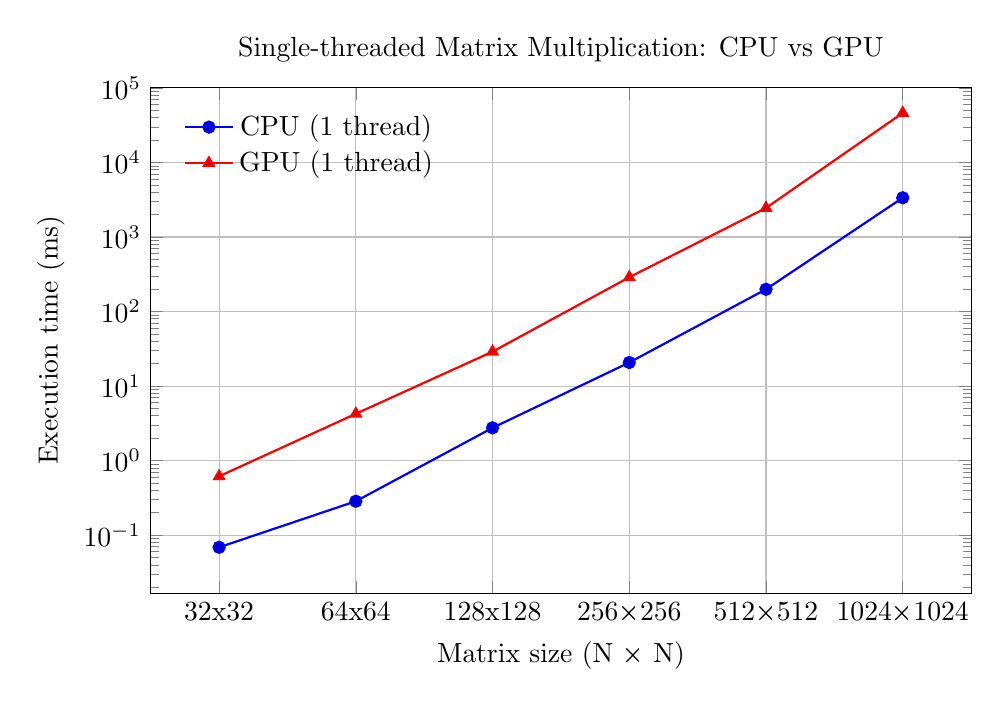
\begin{tikzpicture}
\begin{axis}[
    ymode=log,
    log basis y=10,
    width=12cm,
    height=8cm,
    xlabel={Matrix size (N × N)},
    ylabel={Execution time (ms)},
    title={Single-threaded Matrix Multiplication: CPU vs GPU},
    legend pos=north west,
    xtick=data,
    xticklabels={32x32, 64x64, 128x128, 256×256, 512×512, 1024×1024},
    ymin=0,
    ymax=100000,
    grid=major,
    legend style={draw=none, fill=none}
]

\addplot+[mark=*, thick, blue] coordinates {
    (1, 0.068705)
    (2, 0.285104)
    (3, 2.751817)
    (4, 20.706290)
    (5, 198.716200)
	(6, 3356.762000)
};
\addlegendentry{CPU (1 thread)}

\addplot+[mark=triangle*, thick, red] coordinates {
    (1, 0.615584)
    (2, 4.249685)
    (3, 28.923530)
    (4, 287.943700)
    (5, 2446.466000)
    (6, 46097.410000)
};
\addlegendentry{GPU (1 thread)}

\end{axis}
\end{tikzpicture}

  }
  \caption{Single threaded Matrix Multiplication Execution between CPUs and GPUs averaged over 10 executions}
  \label{fig:singlethreadedgraph}
\end{figure}

\begin{figure}[H]
	\centering
	\resizebox{1.0\linewidth}{!}{
		\begin{tabular}{|r|r|r|r|r|}
\hline
\textbf{Matrix Size (n $\times$ n)} & \textbf{CPU Time (ms)} & \textbf{GPU Time (ms)} & \textbf{Speedup (GPU/CPU)} \\
\hline
32 $\times$ 32     & 0.068705   & 0.615584    & 11.970438 \\
64 $\times$ 64     & 0.285104   & 4.249685    & 15.554119 \\
128 $\times$ 128   & 2.751817   & 28.923530   & 11.419879 \\
256 $\times$ 256   & 20.706290  & 287.933700  & 13.906730 \\
512 $\times$ 512   & 198.716200 & 2446.466000 & 12.323010 \\
1024 $\times$ 1024 & 3356.762000 & 46097.410000 & 13.745850 \\
\hline
\end{tabular}


	}
	\caption{Data Matrix from Figure~\ref{fig:singlethreadedgraph}}
	\label{fig:singlethreadedmatrix}
\end{figure}	




As seen in Figure~\ref{fig:singlethreadedgraph} and Figure~\ref{fig:singlethreadedmatrix} applications that fail to utilize the concurrancy of \acsp{GPU}, either due to programmatical errors or a lack of parallelism in the task, will struggle to achieve high performance.
For each of the matrices tested, through prefetching, a higher clock rate, and branch prediction, the CPU is on average around 13 times faster than the \acs{GPU} running the exact same algorithm. 
Following these results, the \acs{GPU} should only be used in place of the \acs{CPU}, when the application is well tuned to the programming model and a scheduler must respect this difference.
If a \acs{GPU} scheduler is written without regard for these differences, it will may not be able to achieve the desired performance benefit.
This fundamental architectural and programming style for \acsp{GPU} must be understood in order to maximize the throughput. 

\subsection{GPU Hardware Architecture based on the Tesla V100 GPU}


For the purposes of programming and scheduling tasks onto the Tesla V100 GPU\footnote{For the purpose of this thesis, the NVIDIA Tesla V100 GPU chip, which uses the Volta GV100 architecture, was selected due to its availability and high performance computing capabilities.}, the GPU appears as an array of independent highly parallelized processors, called \acsp{SM}.
The \acsp{SM} are grouped into specific \acsp{TPC}, which are then further grouped into \acsp{GPC}, but the specific mapping of tasks to \acs{SM}, \acs{TPC}, and \acs{GPC} is determined by the proprietary hardware scheduler, the GigaThread Engine. 
The exact workings and scheduling methods of the GigaThread Engine are not publicly available, but this module maps \acsp{CTA}, groups of threads executing the same instruction code, to the individual \acsp{SM} based a multitude of factors: hardware resources, parallelism, priorities, and dependencies.
Similarily, the global memory and L2 cache utilization are determined by the hardware and transparent to the programmer.
After the \acs{CTA} gets mapped to the specific \acs{SM}, the device code then executes till completion. 
Each \acs{SM} manages its scheduled \acsp{CTA} through its own execution pipelines, register files, shared memory and scheduling units that function independently from one another. 
For \acsp{SM} to communicate with one another, they must use either the global on-chip device \acs{HBM2} or through the global L2 cache which is shared and coherent across all \acsp{SM}.
Although these memory accesses allows individual \acsp{SM} to communicate with each other, accesses require hundreds of cycles, which introduce further latencies when compared to local \acs{SM} L1 memory caches.
Ideally, the \acsp{SM} execute independently of one another and cumulate answers in global memory, skipping the high memory latency accesses of coordinating synchronous work.

Applications are scheduled to the \acs{SM} by the GigaThread Engine consisting of a \acs{CTA}, or block of threads executing the same instruction code, which then get subdivided into warps to be executed across the \acs{SM}'s execution units.
On the \acs{GPU}, the smallest unit of execution is the Warp, a group of 32 threads that executes instructions in lockstep.
Warps always consist of 32 threads, even if the \acs{CTA} is not divisible by 32 and cannot be fully partitioned across the warps. 
The lockstep execution pattern of warps, enforce that each thread within the warp executes the same instruction, even if several threads are inactive. 
As a consequence, control logic that forces divergent threads significantly slows execution and overutilizes CUDA cores, as the individual threads are forced to execute sequentially.
%If the \acs{CTA} is scheduled with a number of threads indivisible by 32, then the last Warp will still have 32 threads, but the additional threads are deactiveated using a mask.
%Consider the implementation of a program with 33 threads. 
%This application would use 33 software threads, but take up 64 hardware threads with most the CUDA cores assigned by the dispatch unit in the second Warp sitting idle, while the only active thread executes. 

The Tesla V100 GPU \acs{SM} architecture, self contains an entire execution pipeline within each of its 4 processing partitions, which collectively share an L1 instruction cache as well as an L1 data and shared memory cache.
As \acsp{CTA} are distributed across multiple Warps, these collective L1 caches allow the instruction memory and shared memory to be stored across different Warps within the same \acs{CTA}.
The main components of each processing partition are a L0 instruction cache, warp scheduler, dispatch unit, execution units.
Every clock cycle, the Warp scheduler schedules a singular Warp of 32 threads, which get passed to the Dispatch unit. 
The dispatch unit then dispatches a new instruction to the Warp every clock cycle. 
As for any given instruction there are not enough execution units of the same type, the instructions get queued onto the execution units. 
Depending on the current queue and any delays, such as global memory accesses or dependencies, the Warp scheduler will interweave different Warps together onto the Dispatch Unit to hide latencies. 
Within each \ac{SM} processing partition's execution units, there are Tensor Cores for deep learning, 64 bit-\ac{FP} cores, \ac{LD/ST} units, a register file, and \acs{SFU}s for mathematical functions such as sine and square root. 
An in depth view of the processing partition's architecture is provided in Figure~\ref{fig:processing_partition}.



\begin{figure}[H]
  \centering
  \includegraphics[width=0.3\textwidth]{figures/output-006.png}
  \caption{Architecture from the whitepages: https://images.nvidia.com/content/volta-architecture/pdf/volta-architecture-whitepaper.pdf}
  \label{fig:processing_partition}
\end{figure}


The programmer is limited by the hardware constraints of each \acs{SM} and the total number of \acs{SM}.
On the Tesla V100 architecture, there are 80 \acs{SM}, each supporting up to 64 concurrent warps, allowing a maximum of $64 * 32 = 2048$ threads per \acs{SM}.
In total, that leaves a maximum of $80 * 2048 = 163,840$ total threads.
For comparison, the current \acs{CPU} I have, an Intel Tiger Lake (i5-1135G7), has 4 cores, with 2 hardware threads per core supporting a maximum of 8 hardware threads. 
Even server chips such as the Intel Xeon Gold (6148) only supports 20 hardware threads. 
Although the \acs{GPU} oversubscribes the number of Warps and threads, versus the total number of execution units, at a minimum it can still execute $4 * 32 * 80 = 10840$ threads at a time. 
These hardware enforced limits must observed when programming the \acs{GPU}.

\section{GPU Programming using the CUDA API}

NVIDIA has provided an underlying CUDA API to allow programmers to run tasks on the GPU in a heterogenous computing architecture. 
The \acs{GPU}, in this context device, memory is standalone from the \acs{CPU}, in this context host, memory. 
However, the \acs{GPU} execution is dependent on tasks received from the \acs{CPU}.
Given that the device memory is seperate from the host memory, typical \acs{GPU} workloads work by first allocating memory on the device, copying the memory over, executing the program, copying the memory back, and then freeing the device memory.
Typically, the \acs{CPU} uses the \acs{GPU}, by copying the memory over onto the chip, launching the kernel application, and then copying the result from the \acs{GPU} back to the \acs{CPU}.
Although the CUDA API manages the actual underlying steps, the API allows the programmer to specifically program and optimize the \acs{GPU} for their specific task. 

\subsection{Memory and Bandwidth Considerations}

When transfering data from the host, the CUDA API does not have access to the \acs{CPU}'s disk memory and requires the memory to be pinned to the \acs{CPU}'s \acs{RAM}.
While the CUDA runtime can perform this pinning autonomatically, host arrays allocated directly in pinned memory using \lstinline[language=cuda]'cudaMallocHost()' or \lstinline[language=cuda]`cudaHostAlloc()` skip the added step of pinning memory and enable faster transfers. 
Particularily in applications that are bandwidth bottlenecked, this added transfer latency is significant.
If the pinned memory is too large; however, it restricts the memory availability for the programs currently running on the \acs{CPU}, which may degrade performance by forcing the swapping of memory to disk storage. 

In CUDA, understanding how memory is transferred and managed across the host and the device is crucial for optimizing performance.  
For the programmer, the device memory is partitioned into main memory, the \acs{VRAM}, with a size of 16 GB on the Tesla V100 architecture, as well as on chip memory. 
The programmer can decide between three different models of memory management \lstinline[language=cuda]`__constant__`, \lstinline[language=cuda]`__device__`, and \lstinline[language=cuda]`__shared__` memory.
Both constant and device memory are allocated to the global memory, with constant memory only being writeable by the \acs{CPU} and allowing faster access times due to the reduced coherency required.
The shared memory is shared among all warps and threads of a given \acs{SM} in the L1 data and shared memory cache.  
This memory is far more performant than device memory, but limited in size, due to its location on chip.

\subsection{Kernel Launches}

The task of launching and running device code begins from a kernel launch, which passes the function, its parameters, pointers, and the grid and block dimensions to the \acs{GPU}.
Each kernel launch specifies how work is diveded among thread blocks and individual threads. 
Every block is mapped to a \acs{SM} injectively and is constrained by that \acs{SM}'s hardware resources including the number of threads, registers, available warps, and shared memory. 
If there are no available \acs{SM}'s to meet these requirements the kernel launch will fail.
Should the \acs{CTA} or thread block not fully saturate the hardware resources, additional blocks may be scheduled to the same \acs{SM}. 
Each thread and block is assigned unique identifiers, threadIdx and blockIdx, that allow them to determine their position in the execution grid. 
These identifiers are crucial for structuring parallel computations and can be used to optimize memory access patterns. 
For instance, when threads in a warp access consecutive memory locations, the memory accesses can be coalesced into a single transaction, significantly improving memory throughput

The exact syntax is seen below, 


\subsection{CUDA Streams}

CUDA API calls are queued to the \acs{GPU} using cuda streams, which enforce the execution order of tasks.
\lstinline[language=cuda]{cudaStream_t} defines a command queue for the GPU, which is similar to a Linux file pointer in that it returns an index referring to the specific allocated stream.
Each stream allows the queuing of operations such as kernel launches, memory copies, and memory set operations.
Commands submitted to the same stream are executed sequentially in the order they were issued, ensuring deterministic behavior within that stream.
Multiple streams, however, can run concurrently, enabling overlapping execution of kernels and memory operations to maximize GPU utilization and improve overall performance.
By carefully managing streams, developers can optimize task parallelism and resource usage on the GPU.

The Tesla V100 GPU has two seperate hardware copy engines for copying data from the host to the device and back. 
The copy engines support the transfer in both directions, with one engine specifically being allocated for the unidirectional \acs{D2H} transfer and the other for \acs{H2D}.
Using only one stream for multiple kernels fails to maximize the device memory bandwidth. 
For example, consider the launch of two independent kernels, kernel A and kernel B, each

Executing both kernls in the same stream would force kernel B to wait for kernel A to finish before being able to copy memory to the device using the \acs{H2D}


Using different streams, the streams non deterministically execute with respect to one another, except for the default stream. 
\subsection{Synchronization between Streams}

Using multiple streams enables the programmer greater controll over the execution and perform optimization suited to the hardware. 

By default everything goes into stream 0, but operations defined in different streams may execute concurrently.

\pagebreak
% TODO
Real time systems, which rely extensively on machine learning tasks and data processing tasks, Higher data processing performance is vital to autonomous systems, which rely extensively on machine learning tasks and sensor data processing. 
In autonomous systems a multitude of modules require deep learning, a machine learning technique, to automatically extract patterns, such as computer vision, and make decisions \cite{JEON2021167}.
Deep learning, inspired by the structure of the human brain, is composed of layers of numerous interconnected, identical nodes called neural networks.  
Neural network models rely on mathematical operations between different neighboring layers to perform inference, essentially the prediction making or recognition process.
The layers are represented as matrices, which then get multiplied and convoluted with one another and are used by specialized functions, called activation functions, to introduce non-linearity. 
With very large neural networks with thousands or millions of nodes, the inference computation is repetitive and slow. 
The capability to execute these repeptitive workloads concurrently across different dataset makes \acsp{GPU} fundamental to performance in tasks using complex neural networks.  
Furthermore, \acsp{GPU} are necessary to process the data rate produced by high-bandwidth, high-frequency sensors used in autonomous driving. 
The parallelism in \acs{GPU}s makes them the ideal platform over CPUs for deep learning and data processing tasks, tasks fundamental for autonomous driving systems.


Real time systems, such as autonomous driving, are designed with strict timing constraints in mind, to ensure predictable and deterministic behavior \cite{10155700}. 
deadlines, which are subdivided into soft and hard-deadlines. 
Hard deadlines are critical and a failure leads to the systems failure or unsafe conditions. 
For example, in autonomous driving, collision avoidance with another vehicle and brake activation are hard deadlines. 
If these deadlines are not met, the safety of the passengers and the system is at risk. 
On the other hand, soft deadlines are not critical and missing these deadlines degrades performance, but does not cause system failure. 
In autonomous driving, this would show in route planning and navigation updates, where a delay would lead to suboptimal paths, but safety is not comprimised. 
Real time systems need to be capable of effectively and efficiently switching from lower priority tasks, soft deadline tasks, to high priority, hard deadline tasks, to ensure the safety both for the passengers and nearby individuals.  





\subsection{Necessesity of \acsp{GPU} in Autonomous Driving}

\subsection{Autonomous Driving as a Real Time System}

\section{Background}
\subsection{Asynchronous Programming and Coroutines}

Asynchronous programming is a method of programming a system to handle tasks concurrently instead of sequentially. 
Typically used in conjunction with tasks that delay or have high wait-times, such as I/O heavy jobs, asynchronous programming reduces overall execution time by more efficiently using processing ressources. 
For example, while waiting for I/O heavy input like sensor I/O, asynchronous code lets other tasks execute in the meantime, before returning when the data arrives.  
For real-time systems, asynchronous programming additionally uses the intermittant execution model to enforce determinism. 
By allowing the \acsp{GPU} to switch between concurrent tasks, hard deadlines can be immediately enforced without delay. 


Coroutines, an implementation of asynchronous programming, uses suspendable functions to halt execution. 
Suspendable functions are implemented by capturing the current context, know as the continuation, of the currently running thread and save the data to be run later \cite{Zheng2022LuisaRender}. 
After being saved, a new process can take over execution, without interrupting or overwritting the state of the previous process. 
Once the intermittant process or higher priority process has finished execution, the original task can continue executing by restoring the process context, which was previously saved. 
Capturing the continuation of a function allows the resumption of the program to be strategically deferred. 

%Here, the scheduled tasks are independent of the control flow, meaning the execution order of the subtasks





\subsection{NVIDIA Tesla V100 Architecture}


 %\section{Motivation}
 %In autonomous driving and other real time system tasks, GPUs are essential for data processing and machine learning; however,  existing GPU scheduling techniques fail to meet the strict timing requirements of real-time applications.
 %GPU tasks are traditional queued and scheduled based on availabilty to optimize for high throughput applications like graphics rendering and offline machine learning training.
 %These tasks run to completion before switching tasks, meaning multiple tasks, such as the different modules in autonomous driving cannot efficiently share resources. 
 %Depending on the current workload for the GPU, execution times and latency can vary. 
 %These limitations make existing GPU scheduling mechanisms unsuitable for real-time applications like autonomous driving, where deadlines need to be met to ensure the safety of the system and passengers. 

%Citation test~\parencite{latex}.

%Acronyms must be added in \texttt{main.tex} and are referenced using macros. The first occurrence is automatically replaced with the long version of the acronym, while all subsequent usages use the abbreviation.

%E.g. \texttt{\textbackslash ac\{TUM\}, \textbackslash ac\{TUM\}} $\Rightarrow$ \ac{TUM}, \ac{TUM}

%For more details, see the documentation of the \texttt{acronym} package\footnote{\url{https://ctan.org/pkg/acronym}}.




%Autonomous driving system

%In order to react in time to input, autonomous driving systems need to efficiently process 

%By removing human error and utilizing the faster reaction times of computers, autonomous driving can make transportation safer, more accessible, improve traffic efficiency, and reduce the number of traffic accidents.

%For \ac{AVs}, driving tasks rely on complex computations to both understand the surrounding environment and to react to it in real-time.
%Many of these computations are scheduled onto a \ac{\ac{GPU}}, to leverage the high degree of parallelism in the architecture. 
%However, similar to \ac{CPU}s, the \ac{\ac{GPU}} can experience contention when multiple tasks compete for processing power. 
%Unlike \ac{CPU}s, though, \ac{\ac{GPU}}s are less efficient at quickly switching between different tasks, which can lead to delays and unpredictability. 
%If too many tasks get scheduled at once, the system's ability to meet critical deadlines can be comprimised, potentially leading to safety hazards. 
%Using coroutines on persistant threads, \ac{\ac{GPU}} scheduling can be adapted to mitigate contention and ensure real-time system guarantees, enhancing the safety and reliability of \ac{AV}s.


%These autonomous driving modules use vast amounts of data for their computation tasks, which are based in deep learning, a machine learning technique that demands vast amounts of computational resources.
%Deep learning, inspired by the structure of the human brain, utilizes neural networks, with many layers of neural nodes, to automatically extract patterns, enabling decision-making tasks such as classification and object detection.  
%In perception, deep learning models, particularily \acs{CNN}s identify objects, lane markings, pedestrians, vehicles, and traffic lights from the raw sensor data. 
%Beyond perception, deep learning enhances localization by refining sensor fusion techniques, improving accuracy in determining the vehicles position. 
%Furthermore, deep learning also supports planning and control, through reinforcement learning and predictive models to optimize trajectories. 
%The real-time nature of these components are needed to reduce the latency, which requires these models to continously be updating their predictions as new sensor input arrives and the vehicle moves.
%This places a high demand on the hardware, requiring high-performance accelerators to process vast amounts of data efficiently. 
%To meet these requirements, these computations are scheduled on to a \ac{GPU}, which provides the high degree of parallelism required by the vast amount of data and computations within autonomous driving. 



Real time systems, such as autonomous driving, are designed with strict timing constraints in mind, to ensure predictable and deterministic behavior \cite{10155700}. 
They use a concept of deadlines, which are subdivided into soft and hard-deadlines. 
Hard deadlines are critical and a failure leads to the systems failure or unsafe conditions. 
For example, in autonomous driving, collision avoidance with another vehicle and brake activation are hard deadlines. 
If these deadlines are not met, the safety of the passengers and the system is at risk. 
On the other hand, soft deadlines are not critical and missing these deadlines degrades performance, but does not cause system failure. 
In autonomous driving, this would show in route planning and navigation updates, where a delay would lead to suboptimal paths, but safety is not comprimised. 
Real time systems need to be capable of effectively and efficiently switching from lower priority tasks, soft deadline tasks, to high priority, hard deadline tasks, to ensure the safety both for the passengers and nearby individuals.  
